\documentclass[Main]{subfiles}
\begin{document}

\chapter{}
This chapter will cover the fundamentals in data distribution service (DDS), explaining the concept of middleware and DDS for real-time systems.
\section{Middleware}
In distributed systems, where multiple independent computers are connected on a network due to collaborating in achieving the same goal. These computers can be placed with different geographical locations and have different operating systems (OS) \cite[p. 2]{Tanenbaum}.
\\ To make the development of a distributed system easier the developers can use middleware, which is software between the application and the physical layers on the computer. The middleware contributes to the development as it hides the problems that can occur due to different software, hardware and OS's from each application \cite[p. 3]{Tanenbaum}.

\begin{figure}[hbtp]
\centering
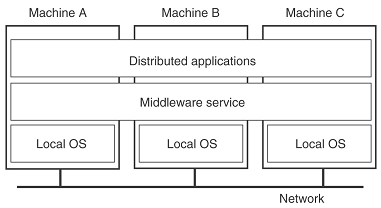
\includegraphics[scale=1]{Figure/Middleware.png}
\caption{A distributed system with middleware \cite[p. 3]{Tanenbaum}}
\label{Fig:Middleware}
\end{figure}

Each application is offered the same interface through the middleware layer which extends over multiple machines \cite[p. 3]{Tanenbaum}. The middleware is a principle that makes it easier for developers to scale a distributed system, as the developer can focus on the interface to the middleware and not the layers beneath. This makes the environment homogeneous as the differences in network technology, hardware architecture, OS, programming languages and geographical locations etc. \cite{DDS-slides} \cite[p. 68]{Coulouris}.
\\
To support the different programming languages used in the applications the middleware supports the Interface Definition Language (IDL). This mean that each application transform the programming langauge into IDL and transfer it into the middleware. The middleware takes care of mapping the IDL
language to the wanted programmering langauge for the given application. \cite{RTI}.
\\
Therefore middleware is useful when developing large and complex distributed systems as it connects the different parts with a "pipe" that makes data-sharing and communication efficient \cite{DDS-slides} \cite[p. 68]{Coulouris}. Also it should be considered that the middleware-software should be installed on all the involved computers which can raise the CPU load. Depending on the type of hardware that is used the developers should choose a sufficient middleware \cite{DDS-slides}.
\\
\\
When choosing between middlewares it is important to know which standard the different middlewares are using. There is a lot of standards that the middleware can support, e.g. which network the middleware supports or if the middleware supports a medical standard for transferring images and data between devices in the medical industry \cite{DDS_slides}.\\
There are various implementations of the standards e.g. OpenDDS by Object Computing Inc. which is an open source implementation. Among the commercial implementations Real-Time Innovations (RTI) has developed a middleware called Connext.

Mia - Skal der skrives mere her? Synes Christian sagde noget men har pt glemt det - ved ikke om du går lidt i dybden med det i dit afsnit? Det var noget de forskelilge standarder, mens synes vi går i dybden med det når vi forklare DDS.
\\\\
A concrete implementation of this middleware in a distributed system, is seen below.
\begin{figure}[hbtp]
\centering
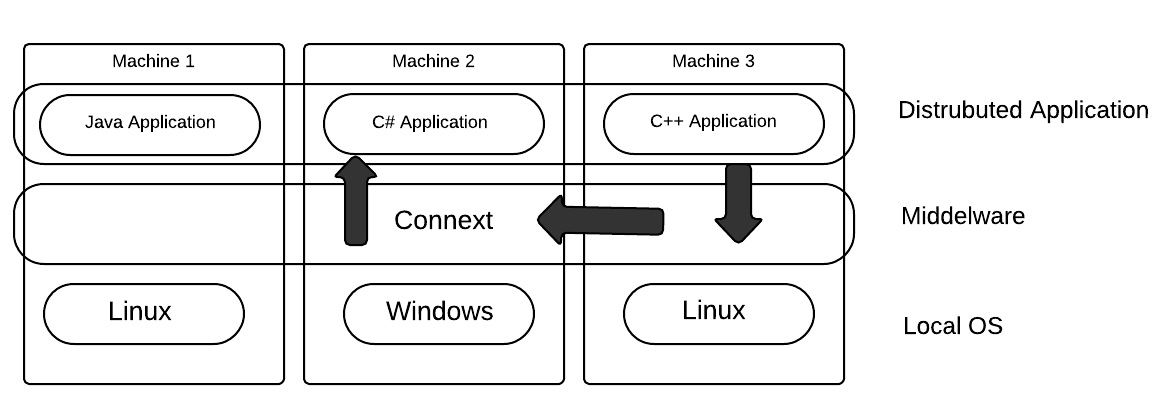
\includegraphics[scale=0.4]{Figure/MiddelwareImplementation.png}
\caption{Connext in a distributed system}
\end{figure}

The figure shows, that a C++ application on Machine 3 is transfered to the middleware. The middleware then handle and transform it, so it can be used on Machine 2, even if the programmering language and the machine is different from each other. 
\\
The communication in the middelware is performed by a publish-subscriper paradigm, called Data-Centric publish-subscripe, which is explained in details in a later section. Other forms of middelware communication paradigms is e.g. Message Passing, Message queuing, Remote procedure call and derivatives and etc.\cite{DDS-slides}.\\
These commuincation paradigms in middelware decouples data producers and consumers in different ways, and they is categorized into 3 different decouplings. These are Space, time and flow decoupling. \\
Space decoupling is if the producers and the consumers dont know each other, which means that they dont got a strong(decideret?) reference to each other. 
\\
Time decoupling is if the interaction is asynchronous, which means that the data being passed can be used later and not when it is recieved. An example on an asyncronous communication could be a mail client which recieves mails, but the mails can be read at a later time then when its arrived. A syncronous communication could be a phone call, where its only possible to talk when another one is calling you. \\
Flow decoupling is if the data production and consumption are not blocking the flow for the producer or the consumer. This means that the producer and the consumer dont block each other when they used the data being passed between them. 

\section{Data distribution service for real-time systems}
The DDS is a specification standard, approved by the Object Management Group (OMG), that facilitates data-communication through the data-centric publish/subscribe paradigm \cite{RTI}. The DDS standard supports deterministic data-delivery (if the underlying data-link and physical layer supports it), a large number of configuration parameters and a low overhead on memory and CPU \cite{DDS-slides}.\\
The specification for DDS consists of two distinct sections; Data Logical Reconstruction Layer (DLRL) and Data-Centric Publish-Subscribe (DCPS) \cite{DDS-slides}.


\begin{figure}[H]
\centering
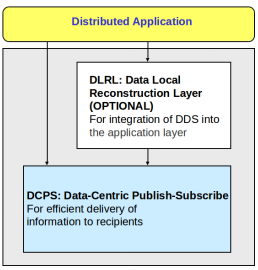
\includegraphics[scale=1]{Figure/DLRLandDCPS.png}
\caption{The two sections in the DDS specification \cite{DDS-slides}}
\label{Fig:DLRL}
\end{figure}

The DLRL is an optional upper layer that allows a simpler integration of the DDS into the application layer. It provide a more natural access to data as it updates a local copy of the data, which allows the application to access the data as if local \cite{DDS-slides}. It outlines how an application can interface with DCPS data fields. According to Gerardo Pardo from RTI no DDS vendors supports the DLRL any more \cite{DLRL-support}.\\
The DCPS is the lower layer which the application uses to communicate with other DDS-enabled applications; it provides efficient delivery of the proper information to the proper recipients \cite{wiki-DDS}. The DCPS comprises the following entities, which can also be seen in Figure ~\ref{Fig:Entities}:
\begin{itemize}
  \item \textbf{Domain}\\The basic construct that binds the individual applications together and where data is send and received from. The domain is the defined communication-area in which the data is being shared.
  \item \textbf{Domain participant}\\This object enables the developer to specify default Quality of Service (QoS) parameters for all entities in the corresponding domain.
  \item \textbf{Data Writer}\\The primary access point for an application to publish data into the data domain. All data that 
  \item \textbf{Publisher}
  \item \textbf{Data Reader}
  \item \textbf{Subscriber}
  \item \textbf{Topic}
  \\\cite{RTI}
\end{itemize}


\begin{figure}[H]
\centering
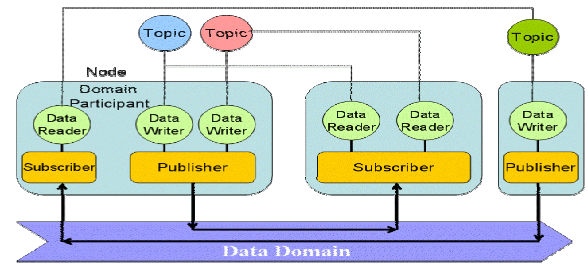
\includegraphics[scale=1]{Figure/DDSentities.png}
\caption{The DDS/DCPS entities \cite{RTI}}
\label{Fig:Entities}
\end{figure}



As described in the section above the RTI Connext implements the DDS standard


\end{document} 